\documentclass{article}
\usepackage{float}
\usepackage{cancel}
\usepackage[T1]{fontenc} % codificação da fonte em 8-bits
\usepackage[utf8]{inputenc} % acentuação direta
\usepackage[brazil]{babel} % em portugues brasileiro
\usepackage[normalem]{ulem}
\useunder{\uline}{\ul}{}
\usepackage{graphicx}
\usepackage[utf8]{inputenc}
\usepackage{fullpage}
\usepackage{listings}
\usepackage{xcolor}
\usepackage{amsmath}
\usepackage{amssymb}
\usepackage{url}
\usepackage{hyperref}
\usepackage[linesnumbered,ruled,vlined]{algorithm2e}
% \usepackage{enumitem}
\usepackage[shortlabels]{enumitem}
\usepackage{listings}
\lstset { %
	language=C++,
	backgroundcolor=\color{black!5}, % set backgroundcolor
	basicstyle=\footnotesize,% basic font setting
}

\definecolor{mygreen}{rgb}{0,0.6,0}

% set the default code style
\lstset{
	language=C++,
	frame=tb, % draw a frame at the top and bottom of the code block
	tabsize=4, % tab space width
	showstringspaces=false, % don't mark spaces in strings
	numbers=none, % display line numbers on the left
	commentstyle=\color{mygreen}, % comment color
	keywordstyle=\color{blue}, % keyword color
	stringstyle=\color{red}, % string color
	backgroundcolor=\color{black!5}, % set backgroundcolor
	basicstyle=\footnotesize,% basic font setting
	literate = {-}{-}1, % <------ trick for '-' in shell commands
}

\parindent0in
\pagestyle{plain}
\thispagestyle{plain}

	
	\title{Trabalho I: Análise bayesiana no caso Normal.}
	\author{Disciplina: Inferência Estatística \\ Aluno: Iara Cristina Mescua Castro}
	
	\begin{document}
		\maketitle
		
		\textbf{Data de Entrega: 24 de Agosto de 2022.}
	
	\paragraph{Questão 1: Escreva a distribuição conjunta condicional dos dados sob a nova parametrização}

	Resposta:\\
	$$f_n ( \underline{x} | \phi ) = \prod_{i = 1}^{n} f( x_i | \phi ) =\prod_{i = 1}^{n} \frac{\sqrt{\tau}}{\sqrt{2 \pi }} e^{-\frac{\tau (x-\mu)^2}{2}}$$

	$$= \left(\sqrt{\frac{\tau}{2 \pi}}\right)^n e^{-\frac{\tau}{2} \sum_{i=1}^{n} (x_{i} - \mu)^2}$$
	
	É possível desconsiderar a constante $(\sqrt{{2 \pi}})^n$:
	
	$$f_n ( \underline{x} | \phi ) \propto \left(\sqrt{\tau}\right)^n e^{-\frac{\tau}{2} \sum_{i=1}^{n} (x_{i} - \mu)^2}$$
	
	\paragraph{Questão 2: A partir da densidade do item anterior, deduza que a distribuição a priori conjugada conjunta para $\phi = (\mu, \tau)$ da forma}
	
	$$ \tau \sim\ Gama(\alpha_0, \beta_0)$$
	$$ \mu | \tau \sim\ Normal(m_0, \lambda_0 \tau)$$
	
	Resposta:\\
	
	A priori de $\tau$:
	$$\xi(\tau) \quad \propto \quad \tau^{\alpha_0 - 1} e^{-\beta_0 \tau}$$
	A priori conjunta de $\mu|\tau$
	$$\xi(\mu | \tau) \quad \propto \quad \sqrt{\tau} \: e^{-\frac{\lambda_0 \tau}{2} (\mu - m_0)^2}$$
	
	$$\xi(\mu | \tau) = \frac{\xi(\mu , \tau)}{\xi(\tau)} \Leftrightarrow \xi(\phi) = \xi(\mu , \tau) = \xi(\mu | \tau) {\xi(\tau)}$$
	
	$$\xi(\phi) = \xi(\mu , \tau) = (\sqrt{\tau} \: e^{-\frac{\lambda_0 \tau}{2} (\mu - m_0)^2}) * (\tau^{\alpha_0 - 1} e^{-\beta_0 \tau}) $$
	
	$$\xi(\phi) \propto (\tau^{\alpha_0 - 1} e^{-\beta_0 \tau}) * (\sqrt{ \tau} \: e^{-\frac{\lambda_0 \tau}{2} (\mu - m_0)^2}) $$
	
	$$\xi(\phi) \propto \tau^{\alpha_0 - 1} e^{-\beta_0 \tau} \sqrt{ \tau} e^{-\frac{\tau}{2}(\lambda_0 (\mu - m_0)^2)}$$
	
	Fórmula para posteriori conjunta:
	$$\xi(\mu, \tau | \underline{x}) \propto \xi(\mu , \tau) \cdot f_n(\underline{x} | \mu, \tau)$$
	$$\xi(\phi | \underline{x}) \propto \xi(\phi) \cdot f_n(\underline{x} | \phi)$$
	
	$$\xi(\phi | \underline{x}) \propto \left(\tau^{\alpha_0 - 1} e^{-\beta_0 \tau} \sqrt{\tau} e^{-\frac{\tau}{2}(\lambda_0 (\mu - m_0)^2} \right) \left(\left(\sqrt{\tau}\right)^n e^{-\frac{\tau}{2} \sum_{i=1}^{n} (x_{i} - \mu)^2} \right)$$
	
	$$\xi(\phi | \underline{x}) \propto \tau^{\alpha_0 + \frac{n}{2} - 1} e^{-\beta_0 \tau} \sqrt{ \tau} e^{-\frac{\tau}{2}(\lambda_0 (\mu - m_0)^2 + \sum_{i=1}^{n}(x_i - \mu)^2)}$$

	Agora precisamos arrumar essa expressão para encontrar uma conjunta de distribuição gama e normal:\\

	
	Vamos rearranjar os índices da segunda exponencial: $e^{-\frac{\tau}{2}(\lambda_0 (\mu - m_0)^2 + \sum_{i=1}^{n}(x_i - \mu)^2)}$
	
	Abrindo os quadrados:
	
	$$-\frac{\tau}{2}(\lambda_0 (\mu^2 - 2\mu + m_0^2) + \sum_{i=1}^{n} xi^2 - 2\sum_{i=1}^{n}x_i \mu + \sum_{i=1}^{n} \mu^2)$$
	
	Agora vamos colocar $\mu^2$ e $- 2\mu$ em evidência. ps.: $\sum_{i=1}^{n}\mu^2 = n \mu^2$ 
	
	$$-\frac{\tau}{2} (\mu^2 (\lambda_0 + n) - 2\mu (\lambda_0 m_0 + \sum_{i=1}^{n}x_i) + \sum_{i=1}^{n}xi^2 + \lambda_0 m_0^2)$$
	
	Colocando $(\lambda_0 + n)$ em evidência em toda a expressão:
	
	$$-\frac{\tau}{2} ((\lambda_0 + n)(\mu^2 - 2 \mu \left(\frac{\lambda_0 m_0 + \sum_{i=1}^{n}x_i}{\lambda_0 + n}\right) + \frac{\sum_{i=1}^{n}x_i}{\lambda_0 + n} + \frac{\lambda_0 m_0^2}{\lambda_0 + n}))$$
	
	Agora é possível completar quadrados de forma que $\omega = \frac{\lambda_0 m_0 + \sum_{i=1}^{n}x_i}{\lambda_0 + n}$:
	
	$$-\frac{\tau}{2} ((\lambda_0 + n)((\mu - \omega)^2 - \omega^2 + \frac{\sum_{i=1}^{n}x_i}{\lambda_0 + n} + \frac{\lambda_0 m_0^2}{\lambda_0 + n})$$
	
	Concluímos que:
	
	$$\xi(\phi | \underline{x}) \propto \tau^{\alpha_0 + \frac{n}{2} - 1} e^{-\beta_0 \tau - \frac{\tau}{2} (\sum_{i=1}^{n}x_i^2 + \lambda_0 m_0^2 - \cancel{\lambda_0 + n} \left(\frac{(\lambda_0 m_0 + \sum_{i=1}^{n}x_i)^2}{(\lambda_0 + n)^{\cancel{2}}}\right))} \sqrt{\tau} e^{-\frac{\tau}{2}(\lambda_0 + n)(\mu - \omega)^2}$$
	
	$$\xi(\phi | \underline{x}) \propto \tau^{\alpha_0 + \frac{n}{2} - 1} e^{-\beta_0 \tau - \frac{\tau}{2} (\sum_{i=1}^{n}x_i^2 + \lambda_0 m_0^2 - \frac{(\lambda_0 m_0 - \sum_{i=1}^{n}x_i)^2}{\lambda_0 + n}}  \sqrt{\tau} e^{-\frac{\tau}{2}(\lambda_0 + n)(\mu - \omega)^2}$$
	
	$$\xi(\phi | \underline{x}) \propto \tau^{(\alpha_0 + \frac{n}{2}) - 1} e^{-\tau (\beta_0 + \frac{1}{2} (\sum_{i=1}^{n}x_i^2 + \lambda_0 m_0^2 - \frac{(\lambda_0 m_0 - \sum_{i=1}^{n}x_i)^2}{\lambda_0 + n})} \sqrt{\tau} e^{-\frac{\tau}{2}(\lambda_0 + n)(\mu - \omega)^2}$$
	
	Note que a primeira parte depende apenas de $\tau$, enquanto a segunda parte (a partir de $\sqrt{\tau}$) depende de $\mu$ e $\tau$.
	
	Sabendo que $\xi(\mu, \tau) = \xi(\tau) \xi(\mu | \tau) \Leftrightarrow \xi(\phi) = \xi(\tau) \xi(\mu | \tau)$ 
	
	$$\xi(\phi | \underline{x}) = \xi(\tau | \underline{x}) \xi(\mu | \tau, \underline{x})$$
	Podemos concluir que:  
	
	$$\xi(\tau | \underline{x}) = \tau^{(\alpha_0 + \frac{n}{2} - 1)} e^{-\tau (\beta_0 + \frac{1}{2} (\sum_{i=1}^{n}x_i^2 + \lambda_0 m_0^2 - \frac{(\lambda_0 m_0 - \sum_{i=1}^{n}x_i)^2}{\lambda_0 + n})}$$
	
	$$ \xi(\mu | \tau, \underline{x}) = \sqrt{\tau} e^{-\frac{\tau}{2}(\lambda_0 + n)(\mu - \omega)^2}$$
	
	\paragraph{Questão 3: A partir dos itens anteriores, derive a distribuição a posteriori conjunta de
		$\mu$ e $\tau$ e a distribuição conjunta de $\mu$ dado $\tau$, assim como a distribuição marginal a posteriori de $\tau$}.
	
	A partir da questão anterior, obtemos que:
	
	$$\xi(\phi | \underline{x}) \propto \underbrace{\tau^{(\alpha_0 + \frac{n}{2}) - 1} e^{-\tau (\beta_0 + \frac{1}{2} (\sum_{i=1}^{n}x_i^2 + \lambda_0 m_0^2 - \frac{(\lambda_0 m_0 - \sum_{i=1}^{n}x_i)^2}{\lambda_0 + n})}}_{1} \underbrace{\sqrt{\tau} e^{-\frac{\tau}{2}(\lambda_0 + n)(\mu - \omega)^2}}_{2}$$
	
	É proporcional às duas distribuições: 
	
	1) $\xi(\tau | \overline{x}) = Gama(\alpha_1, \beta_1)$, onde:\\
	
	$\alpha_1 = \alpha_0 + \frac{n}{2}$ e $\beta_1 = \beta_0 + \frac{1}{2} (\sum_{i=1}^{n}x_i^2 + \lambda_0 m_0^2 - \frac{(\lambda_0 m_0 - \sum_{i=1}^{n}x_i)^2}{\lambda_0 + n})$\\
	
	 
	2) $\xi(\mu | \tau, \overline{x}) = Normal(m_1, \lambda_1)$, onde:\\
	
	$m_1 = \omega = \frac{\lambda_0 m_0 + \sum_{i=1}^{n}x_i}{\lambda_0 + n}$ e $\lambda_1 = \lambda_0 + n$\\
	
	-------------------------------------------------------------------------------------------------------------------------
	

	
	\paragraph{Questão 4: Interprete as expressões obtidas no item anterior; o que as formas funcionais
	obtidas revelam sobre a interação entre os hiperparâmetros e os dados?}.\\

	Elas revelam que devido o $\lambda_0$ em uma pequena quantidade de amostras, faz a distribuição ser mais espalhada já que a variância aumenta. Isso se dá por ser inversamente proporcional à $\xi(\mu | \tau, \overline{x})$. Enquanto em uma grande quantidade de amostras ocorre o contrário, a variância é menor e a distribuição se torna mais concentrada.

	Vale ressaltar também que:
	$$m_1 = \frac{\lambda_0 m_0 + n \overline{x}}{\lambda_0 + n} = \frac{\lambda_0}{\lambda_0 + n} m_0 + \frac{n}{\lambda_0 + n} \overline{x}$$
	
	Então $m_1$ é uma média ponderada da média a priori y da média amostral
	
	$$\frac{\lambda_0}{\lambda_0 + n} + \frac{n}{\lambda_0 + n} = 1$$
	
	$\lambda_1 = \lambda_0 + n \Rightarrow \underbrace{\tau \lambda_1}_{precisao \; condicional} = \underbrace{t\lambda_0}_{precisao \; priori} + \underbrace{\tau n}_{precisao \; amostral}$ 
	\paragraph{Questão 5: Derive a distribuição marginal a posteriori de $\tau$ (Dica: leia o capítulo 8.4
		de De Groot)}.\\
	
	A distribuição marginal a posteriori de $\tau$:
	
	$$ \int_{a}^{b} \xi(\mu, \tau | \underline{x}) \,d\mu = \int_{a}^{b} \xi(\tau | \underline{x}) \xi(\mu | \tau, \underline{x}) \,d\mu $$
	
	Como já foi calculado:
	
	$$= \int_{0}^{\infty} \tau^{\alpha_1 - 1} e^{-\tau \beta_1} \sqrt{\tau} e^{-\frac{\tau}{2}(\lambda_1)(\mu - m_1)^2} d\tau$$
	
	$$= \int_{0}^{\infty} \tau^{\alpha_1 + \frac{1}{2} - 1} e^{-\frac{\tau}{2}(2 \beta_1 + (\lambda_1)(\mu - m_1)^2)} d\tau$$ 
	
	$$= \int_{0}^{\infty} \tau^{\alpha_1 + \frac{1}{2} - 1} e^{-\tau(\beta_1 + \frac{(\lambda_1)}{2}(\mu - m_1)^2)} d\tau$$
	----------------------------------------------------------------------------------------------------------------------------------------
	
	A partir da função Gamma:
	
	$$\Gamma(\alpha) = \int_{0}^{\infty} x^{\alpha - 1} e^{-x}$$
	
	$$\beta x = y \Longleftrightarrow x = \frac{y}{\beta} \Longleftrightarrow \beta dx = dy$$
	
	$$\int_{0}^{\infty} x^{\alpha - 1} e^{-\beta x} dx = \int_{0}^{\infty} \frac{y}{\beta}^{z-1} e^{-y} \frac{1}{\beta} dy$$
	
	$$= \int_{0}^{\infty} \frac{1}{\beta^\alpha} y^{\alpha - 1} e^{-y} dy$$
	
	$$\int_{0}^{\infty} x^{\alpha - 1} e^{-\beta x} dx = \frac{\Gamma({\alpha})}{\beta^{\alpha}}$$
	
	----------------------------------------------------------------------------------------------------------------------------------------
	
	Então:
	
	$$= \int_{0}^{\infty} \tau^{\overbrace{(\alpha_1 + \frac{1}{2})}^{\alpha_2} - 1} e^{-\tau\overbrace{(\beta_1 + \frac{(\lambda_1)}{2}(\mu - m_1)^2)}^{\beta_2}} d\tau = \int_{0}^{\infty} \tau^{\alpha_2 - 1} e^{- \beta_2 \tau} d\tau$$
	
	
	$$\frac{\Gamma(\alpha_1 + \frac{1}{2})}{(\beta_1 + \frac{(\lambda_1)}{2}(\mu - m_1)^2)^{(\alpha_1 + \frac{1}{2})}} \propto (\beta_1 + \frac{(\lambda_1)}{2}(\mu - m_1)^2)^{-(\alpha_1 + \frac{1}{2})}$$
	
	
	$$\xi(\mu | \underline{x}) \propto (\beta_1 + \frac{(\lambda_1)}{2}(\mu - m_1)^2)^{-(\alpha_1 + \frac{1}{2})}$$
	
	$$\xi(\mu | \underline{x}) \propto (1 + \frac{(\lambda_1)}{2 \beta_1}(\mu - m_1)^2)^{-(\frac{2\alpha_1 + 1}{2})}$$
	
	
	Podemos representá-la na forma da distribuição de T-Student, com os parâmetros de locação $m_1$, escala $\frac{2\beta}{\lambda_1}$ e $2 \alpha_1 = 2\alpha_0 + n$ graus de liberdade.
	
	Em outras palavras:
	
	$$\xi(\mu | \underline{x}) \sim\ T-Student(v, \mu, \sigma)$$
	
	$$\xi(\mu | \underline{x}) \sim\ T-Student(2 \alpha_1, m_1, \frac{2\beta_1}{\lambda_1})$$
	
	$$\xi(\mu | \underline{x}) \sim\ T-Student(2 \alpha_0 + n, \frac{\lambda_0 m_0 + \sum_{i=1}^{n}x_i}{\lambda_0 + n}, \frac{2\beta_1}{\lambda_1})$$
	
	Onde $\beta_1 = \beta_0 + \frac{1}{2} (\sum_{i=1}^{n}x_i^2 + \lambda_0 m_0^2 - \frac{(\lambda_0 m_0 - \sum_{i=1}^{n}x_i)^2}{\lambda_0 + n})$ e $\lambda_1 = \lambda_0 + n$
	

	\paragraph{Questão 6: Palmirinha anda preocupada com a concentração de amido em sua pamonha.
		Ela pede para Valciclei, seu assistente, amostrar n = 10 pamonhas e
		medir sua concentração de amido.
		Ele, muito prestativo, rapidamente faz o experimento, mas, porque comeu
		todas as amostras depois que foram medidas, precisou fazer uma visita de
		emergência ao banheiro. Desta feita, apenas teve tempo de anotar em um
		papel a média e variância amostrais, $\overline{x_n}$ = 8.307849 e $\overline{s_n}^2$ = 7.930452.
		Palmirinha tem uma reuni~ao com investidores em pouco tempo, então decide
		voltar aos seus tempos de bayesiana old school e analisar os dados
		utilizando prioris conjugadas. Ela supõe que a concentração de amido segue
		uma distribuição normal com parâmetros $\mu$ e $\tau$ e que as observações
		feitas por Valciclei são independentes entre si. Ela suspeita que a concentra
		ção de amido na pamonha que em torno de 10 mg/L, com desvio
		padrão de 2 mg/L. Com sua larga experiência na confecção de pamonhas,
		ela suspeita ainda que o coeciente de variação da concentração de amido
		seja em torno de 1=2. Palmirinha tem um quadro em seu escritório, que
		diz}
	
		\[ \operatorname{cv} = \frac{\sigma}{\mu}. \]
		
		Agora, 
		
			a) Elicite uma distribuição a priori conjugada consistente com as suspeitas de Palmirinha. Para isso, interprete-as como valores esperados a priori dos parâmetros\footnote{As leis de esperança e de variância totais podem ser adequadas; veja \cite[Seção 9.6]{Blitzstein2019-qi}.}  -- isto é, $\mathbb{E}[\mu] = 10$, $\mathrm{Var}(\mu) = 4$ e $\mathbb{E}[\sqrt{\tau} \mu] = 2$ -- e compute os hiperparâmetros $\beta_{0}$, $m_{0}$ e $\lambda_{0}$ da Equação(1). Suponha também que $\alpha_{0} = 2$.
			
			b) Com os dados anotados por Valciclei, é possível computar a distribuição~\textit{a posteriori} de $\mu$ e $\tau$? Justifique.
			 
			c) Em caso afirmativo, ajude Palmirinha a encontrar $a, b \in \mathbb{R}$, $a < b$ de modo que $\operatorname{Pr}(\mu \in (a, b) \mid \boldsymbol{x}) = 0.95$.
		
		----------------------------------------------------------------------------------------------------------------------------------------\\
		a) $\alpha_0 = 2$, $\beta_0 = ?$, $m_0 = 10$ e $\lambda_0 = ?$\\
		$E[\mu] = 10$, $Var(\mu) = 4$ e $E[\sqrt{\tau}\mu] = 2$
		
		$$E[X] = E[E[X|Y]]$$
		$$Var(X) = Var(E[X|Y]) + E[Var(X|Y)]$$
		
		$$\mu | \tau \sim\ N(m_0, \lambda_0 \tau)$$
		
		$$E[\mu | \tau] = m_0$$		
		$$E[\mu] = E[E[\mu | \tau]] = E[m_0] = m_0$$
		$$m_0 = 10$$
		
		$$Var(\mu) = Var(E[\mu|\tau]) + E[Var(\mu | \tau)]$$
		$$= \cancel{Var(m_0)} + E[\frac{1}{\lambda_0 \tau}] = \frac{1}{\lambda_0} E[\frac{1}{\tau}]$$
		
		$$\tau \sim\ Gamma(\alpha_0, \beta_0)$$
		$$\frac{1}{\tau} \sim\ GammaInverse(\alpha_0, \beta_0)$$
		
		$$= \frac{1}{\lambda_0} \frac{\beta_0}{\alpha_0 - 1} = \frac{\beta_0}{(2-1)\lambda_0} = 4$$
		
		$$\beta_0 = 4 \lambda_0$$
		----------------------------------------------------------------------------------------------------------------------------------------\\
		$$E[E[\sqrt{\tau}\mu | \tau]] = E[\sqrt{\tau} E[\mu | \tau]] = m_0 E[\sqrt{\tau}] = 2$$
		
		----------------------------------------------------------------------------------------------------------------------------------------\\
		
		$$E[\sqrt{\tau}] = \int_{0}^{\infty} \sqrt{\tau} E[\tau] d\tau$$
		
		$$= \frac{\beta_0^{\alpha_0}}{\Gamma(\alpha_0)}  \int_{0}^{\infty} \tau^{\frac{1}{2}} \tau^{\alpha_0 - 1} e^{-\beta_0 \tau} d\tau$$
		
		$$= \frac{\beta_0^{\alpha_0}}{\Gamma(\alpha_0)}  \int_{0}^{\infty} \underbrace{\tau^{(\alpha_0 + \frac{1}{2}) - 1} e^{-\beta_0 \tau}}_{gamma(\alpha_0 + \frac{1}{2}, \beta_0)} d\tau$$
		
		$$= \frac{\beta_0^{\alpha_0}}{\Gamma(\alpha_0)} \frac{\Gamma(\alpha_0 + \frac{1}{2})}{\beta^{\alpha_0 + \frac{1}{2}}}$$
		
		Sabendo que $\alpha_0 = 2$:
		
		$$= \frac{1}{\beta_0^{\frac{1}{2}}} \frac{\Gamma(2 + \frac{1}{2})}{\Gamma(2)}$$
		
		$\Gamma(2) = (2-1)! = 1$
	
		$$= \Gamma(\tfrac{5}{2}) = \frac{3}{2} \Gamma(\tfrac{3}{2}) = \frac{3}{4} \Gamma(\tfrac{1}{2}) = \frac{3 \pi}{4}$$
		
		----------------------------------------------------------------------------------------------------------------------------------------\\
		
		$$E[E[\sqrt{\tau}\mu | \tau]] = \frac{3\sqrt{\pi}}{4} \frac{m_0}{\beta_0^{\frac{1}{2}}} = 2$$
		
		Sabendo que $m_0 = 10$:
		
		$$\frac{3 \sqrt{\pi}}{4} \frac{10}{\sqrt{\beta_0}} = 2$$
		
		$$\frac{3 \sqrt{\pi}}{2} \frac{5}{\sqrt{\beta_0}} = 2$$
		
		$$15 \sqrt{\pi} = 4\sqrt{\beta_0} \Leftrightarrow \beta_0 = \frac{225 \pi}{16}$$
		
		$$\beta_0 = 4 \lambda \Rightarrow \lambda = \frac{225 \pi}{64}$$
		
		----------------------------------------------------------------------------------------------------------------------------------------\\
		b) Sim, para calcular as distribuições a posteriori, precisamos além dos hiper-parâmetros, a média e a variança, que foram dadas.\\
		----------------------------------------------------------------------------------------------------------------------------------------\\
		c) $\mu_{\overline{x}} \sim\ t-student(v, M, \sigma)$\\
		
		$T/\sqrt{\sigma} + M = \mu_{\overline{x}}$\\
		
		$T = (\mu_{\overline{x}} - M)\sqrt{\sigma} \sim\ t(v)$\\
		
		$$P(a < \mu < b | \underline{x}) = 0.95$$	
		$$P(a - M) \sqrt{\sigma} < \underbrace{\overbrace{(\mu - M)}^{T} \sqrt{\sigma}}_{t-student(v)} < (b - M) \sqrt{\sigma}$$
		
		
		\begin{figure}[H]
			\centering
			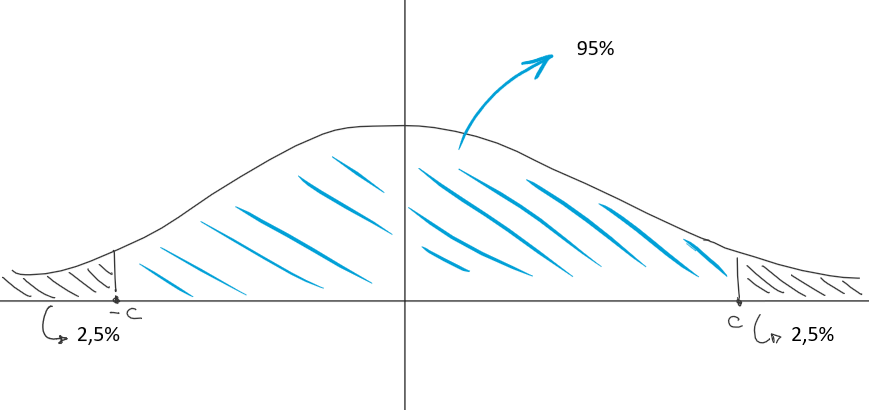
\includegraphics[width=0.6\linewidth]{grafico1}
		\end{figure}
	
	$$(a - M) \sqrt{\sigma} = CumulativeInverse \; t-Student(v) [2,5\%]$$
	$$(b - M) \sqrt{\sigma} = CumulativeInverse \; t-Student(v) [97,5\%]$$
	
	$$a = \frac{t_{2,5}}{\sqrt{\sigma}} + M$$
	
	$$b = \frac{t_{97,5}}{\sqrt{\sigma}} + M$$
	
	Visto que $\alpha_0 = 2$ e $n = 10$:
	$$v = 2\alpha_0 + n = 2 * 2 + 10 = 14$$
	
	$$M = \frac{\lambda_0 m_0 + n \overline{x}}{\lambda_0 + n}$$
	
	Visto que $\overline{x_n} = 8.307849$, $\lambda_0 = \frac{225\pi}{64}$
	
	$$M = \frac{\frac{225\pi}{64} * 10 + 10 * 8.307849}{\frac{225\pi}{64} + 10}$$
	
	$$M = \frac{11.04466 * 10 + 83.07849}{11.04466 + 10} = \frac{193,52509}{21.04466} \approx 9.19$$
	
	
	%$$T = \frac{(\lambda_0 + n)(\alpha_0 + \frac{n}{2})}{\beta}$$
	
	$$\sigma^2 = \frac{\beta}{(\lambda_0 + n)(\alpha_0 + \frac{n}{2})}$$
	
	Como foi visto na questão 2:
	$$\beta = \beta_0 + \frac{1}{2} (\sum_{i=1}^{n}x_i^2 + \lambda_0 m_0^2 - \frac{(\lambda_0 m_0 - \sum_{i=1}^{n}x_i)^2}{\lambda_0 + n}) = \beta_0 + \frac{1}{2} s_n^2 (n-1) + \frac{n \lambda_0(\overline{x} - m_0)^2}{2(\lambda_0 + n)}$$
	
	Substituindo os valores:	
	$$\beta = \frac{225\pi}{16} + \frac{7.930452 * 9}{2} + \frac{10 \frac{225\pi}{64}(8.307849 - 10)^2}{2(21.04466)}$$
	
	$$\beta = 44.1786 + 35.687034 + \frac{\frac{2250\pi}{64}(2.8633)}{42.08932} = 44.1786 + 3.965226 + \frac{316.25}{42.08932}$$
	
	$$\beta = 44.1786 + 35.687034 + \frac{316.25}{42.08932} = 44.1786 + 3.965226 + 7.5137 \approx 87.379334$$
	
	$$\frac{1}{\sigma^2} = \frac{87.379334}{(\frac{225\pi}{64} + 10)(2 + 5)} = \frac{87.379334}{(21.04466)(7)} = \frac{87.379334}{147.31262}\approx 0.5931$$
	
	$$\frac{1}{\sigma} \approx 0.77$$\\
	
	Então temos uma distribuição $t \sim\ T-Student(14, 9.19, \frac{1}{0.77})$
	
	Pela tabela da distribuição t-student, $t_{2.5}$ e $t_{97.5}$ para v = 14 é: $2.14479$: 
	
	Agora podemos calcular $a$ e $b$:
	
	$$a \approx -2.14479 * 0.77 + 9.19 = -2.7854 + 9.19 = 7.5385$$
	
	$$b\approx 2.14479 * 0.77 + 9.19 = 2.7854 + 9.19 = 10.841$$
	 
	\newpage 
	
	\section{Referência Bibliográfica}
	
	Degroot, Schervish. Probability and Statistics 4th Edition, 2011.
	
\end{document}
